\chapter{Coq}\label{ch:coq}

En este capitulo introduciremos las características más relevantes del asistente de pruebas interactivo Coq. El objetivo de este capitulo es introducir todos los conceptos que utilizaremos más adelante, pero esto significa que no es una introducción completa.

El desarrollo de Coq comenzó en 1984 con el apoyo de INRIA como el trabajo de Gérard Huet y Thierry Coquand. En ese momento Coquand estaba implementado un lenguaje llamado \emph{Calculus of Constructions} \cite{DBLP:journals/iandc/CoquandH88}.
En 1991, Coquand creo una derivación del trabajo anterior, \emph{Calculus of Inductive Constructions} \cite{CIC}. Esta teoría comenzó a ser desarrollada y finalmente llegando a ser Coq.

Ahora mismo Coq es desarrollado por más de 40 personas de forma activa y es reconocido como unos de los asistentes de prueba principales.

Como un asistente de pruebas, la orientación de Coq es la de permitir la escritura totalmente formal de teoremas y pruebas, y asegurarnos de su correción. Se parte de lo que se denomina \textit{kernel}, el núcleo de Coq, que es el que verifica que la prueba corresponde al teorema, es decir, que sea correcta. De esta forma, el humano no está encargado de verificar la prueba, solo de escribirla.

El ejemplo más conocido de formalización en Coq es el teorema de los cuatro colores \cite{DBLP:conf/ascm/Gonthier07} hecho por \citeauthor{DBLP:conf/ascm/Gonthier07} en \citeyear{DBLP:conf/ascm/Gonthier07}.

\section{Los lenguajes Coq}

Coq no es técnicamente un lenguaje de programación, sino, un asistente de pruebas. Pero podemos encontrar múltiples lenguajes dentro de Coq que nos permiten expresarnos. 
\begin{description}
    \item[Gallina] Este es el lenguaje de especificación de Coq \cite{Gallina}. Permite desarrollar teorías matemáticas y probar especificaciones de programas. Utilizaremos extensivamente un lenguaje muy similar a este para definir nuestros programas en \Mtac.
    \item[Ltac] El lenguaje en que se definen las \textit{tácticas} de Coq. Es el metalenguaje por defecto de Coq. Introducido por \citeauthor{DBLP:conf/lpar/Delahaye00} en Coq 7.0. Ltac \cite{DBLP:conf/lpar/Delahaye00} es central en Coq y hasta algunos lo consideran una de las principales razones del éxito de este. Antes de Ltac, los usuarios de Coq tenían que escribir los \textit{proof terms} a mano, o sino, utilizaban un conjunto de tácticas muy primitivas que ejecutaban reglas muy básicas. Ltac le proporcionó a los usuarios una forma de escribir sus propias tácticas al unir las tácticas básicas gracias a un conjunto expresivo de combinadores, así permitiendo el desarrollo de formalizaciones más complejas en Coq.
    \item[Vernacular] Este lenguaje contiene los comandos básicos de Coq con los que nos comunicamos con intérprete. En lo que resta del trabajo utilizaremos varios de estos comandos.
\end{description}

Aunque Coq no es un lenguaje de programación propiamente dicho, este puede ser utilizado como un lenguaje de programación funcional. Estos programas serán especificados en Gallina. Dada la naturaleza de Coq como ``probador de teoremas'', estos programas son funciones puras, es decir, no producen efectos secundarios y siempre terminan.

\section{La teoría de Coq}

\textit{Calculus of Inductive Constructions} \cite{CIC} es la base de Coq. Este es un cálculo lambda tipado de alto orden y puede ser interpretado como una extensión de la correspendencia Curry-Howard.

Llamaremos \textit{Terms} (o términos) a los elementos básicos de esta teoría. Terms incluye \textit{Type}, \textit{Prop}, variables, tuplas, funciones, entre otros. Estás son algunas de las herramientas que utilizaremos para escribir nuestros programas.

\section{Tipos de datos y Funciones}

Ahora aprenderemos a codificar nuestros programas funcionales en Coq. Lo primero que debemos entender es que operamos sobre \textit{términos} y algo es un término si tiene tipo. Coq provee muchos tipos predefinidos, por ejemplo \lstinline{unit}, \lstinline{bool}, \lstinline{nat}, \lstinline{list}, entre otros. A continuación estudiaremos cómo definir tipos y funciones.

Veamos cómo se define el tipo \lstinline{bool}:

\begin{lstlisting}
Inductive bool : Set :=
  | true : bool
  | false : bool.
\end{lstlisting}

Como podemos observar, es un tipo inductivo, especificado por el comando \lstinline{Inductive} de Vernacular, con dos constructores \lstinline{true} y \lstinline{false}. De por sí, el tipo \lstinline{bool} no posee un significado hasta que nosotros lo proveamos de uno. Podemos ahora intentar definir algunos operadores booleanos.
\begin{lstlisting}
Definition andb (b1 b2:bool) : bool := if b1 then b2 else false.
Definition orb (b1 b2:bool) : bool := if b1 then true else b2.
Definition implb (b1 b2:bool) : bool := if b1 then b2 else true.
Definition negb (b:bool) := if b then false else true.
\end{lstlisting}

Las definiciones de funciones no recursivas comienzan con el comando \lstinline{Definition}. La primera se llama \lstinline{andb} y toma dos booleanos como argumentos, retornando un booleano. Se utiliza la notación \lstinline{(if b then x else y)} para matchear sobre los booleanos de manera más fácil. Finalmente podemos definir una función más interesante.

\begin{lstlisting}[frame=tb,caption={Definición de \lstinline{is_true}},label=lst:Is_true]
Definition is_true (b:bool) : Prop :=
  match b with
    | true => True
    | false => False
  end.
\end{lstlisting}

La definición de \ref{lst:Is_true} es muy importante. Nos muestra claramente que \lstinline{true} y \lstinline{True} no son lo mismo. Como vimos, \lstinline{true} representa el valor de verdad booleano. Mientras que \lstinline{True} representa la verdad en las proposiciones, es decir, algo que siempre tiene una prueba. De la misma forma, \lstinline{False} representa a los teoremas que nunca podremos probar. En caso de probar \lstinline{False}, sin ninguna hipótesis, estaríamos mostrando que Coq es \emph{inconsistente}.

Ahora, veamos un tipo inductivo recursivo.

\begin{lstlisting}
Inductive nat : Set :=
  | O : nat
  | S : nat -> nat.
\end{lstlisting}

Notemos que el constructor \lstinline{S} es una función que recibe un término de tipo {nat}, es decir, \lstinline{nat} es un tipo \emph{recursivo}, a diferencia de \lstinline{bool}. Por ejemplo, el término \lstinline{S (S O)} es de tipo \lstinline{nat} y representa al número 2.

Para continuar con este desarrollo, veamos el tipo de \lstinline{list} que, aparte de ser recursivo, es polimórfico.

\begin{lstlisting}
Inductive list (A : Type) : Type :=
  | nil : list A
  | cons : A -> list A -> list .
\end{lstlisting}

Este tipo es un tipo polimórfico dado que requiere de un \lstinline{A : Type} para ser un tipo. Antes de conocer ese \lstinline{A}, \lstinline{list} es una función. Por ejemplo, una posible lista es \lstinline{cons (S O) \; nil : list nat} que representa a la lista con un único elemento 1 de tipo \lstinline{nat}.

Definiremos una función que añade un elemento a una lista.

\begin{lstlisting}
Definition add_list {A} (x : A) (l : list A) : list A :=
  cons x l.
\end{lstlisting}

Dado que el tipo \lstinline{A} puede ser inferido fácilmente por Coq, utilizamos llaves a su alrededor para expresar que sea un argumento implícito. En el cuerpo de la función solo utilizamos \lstinline{cons}, uno de los constructores de \lstinline{list}, para añadir un elemento delante de \lstinline{l}.

Ahora nos interesa definir la función \lstinline{len} que retorna el largo de una lista.

\begin{lstlisting}
Fixpoint len {A} (l : list A) : nat :=
match l with
| [] => O
| x :: xs => S (len xs)
end.
\end{lstlisting}

Coq está diseñado de forma que necesitamos utilizar el comando \lstinline{Fixpoint} para poder definir funciones recursivas. Recordemos que las funciones en Coq son puras. Aquí Coq está encontrando el argumento decreciente de la función \lstinline{len}, asegurándose de la terminación de \lstinline{len}.
El cuerpo de la función inspecciona a \lstinline{l} y lo \textit{matchea} con el caso correspondiente. Utilizamos \lstinline{S} y \lstinline{O}, los constructores de \lstinline{nat}, para expresar el valor de retorno.

\section{Tipos dependientes}

Una de las herramientas más importantes de Coq son los tipos dependientes. Estos nos permiten hablar de elementos que dependen de otros anteriores. Por ejemplo, puede ser de nuestro interés hablar de números positivos, más formalmente, \lstinline{x : nat} tal que \lstinline{x <> O}. En este caso, \lstinline{x <> O} es una prueba que depende de \lstinline{x} y solo existirá cuando \lstinline{x} sea mayor a cero.

Para hablar de un ejemplo práctico de tipos dependientes, hemos elegido la función \lstinline{head} que retorna la cabeza de una lista. Comencemos con la versión más simple, donde utilizamos un valor ``default'' \lstinline{d} para el caso en que la lista sea vacía.

\begin{lstlisting}
Definition head_d {A} (l : list A) (d : A) : A :=
  match l with
  | [] => d
  | x :: xs => x
  end.
\end{lstlisting}

El problema de esta solución es que a excepción de que \lstinline{d} sea un valor único o reservado, no hay manera de saber si la función retornó realmente la cabeza de la lista.

La segunda opción es utilizar el tipo \lstinline{option}. Este tipo tiene dos constructores, uno que nos permite guardar un valor y otro que representa el error. De esta forma podemos escribir la siguiente función.

\begin{lstlisting}
Definition head_o {A} (l : list A) : option A :=
  match l with
  | [] => None
  | x :: xs => Some x
  end.
\end{lstlisting}

Esta solución es mejor que la anterior pero sigue sufriendo de una deficiencia. Dado que \lstinline{head_o} retorna un \lstinline{option} no sabemos si el resultado de esta función será realmente un elemento o si será el constructor vacío, por lo que todas las funciones que utilicen a \lstinline{head_o} deben también utilizar \lstinline{option}.

Esto nos lleva a nuestra última solución. Esta requiere que nos aseguremos que la lista \lstinline{l} no es vacia, es decir, \lstinline{l <> []}. Pero para entenderla debemos ver dos cosas más: $\Sigma$\textit{-types} y \lstinline{Program}.
Intuitivamente, los $\Sigma$\textit{-types} son tuplas donde el argumento de la derecha es dependiente del de la izquierda. También podemos llamarlos pares dependientes. A continuación, la definición.

\begin{lstlisting}[frame=tb,caption={Definición de $\Sigma$\textit{-types}},label=lst:sigma-types]
Inductive sig (A : Type) (P : A -> Prop) : Type :=
  exist : \forall x : A, P x -> {x : A | P x}
\end{lstlisting}

Se utiliza la notación \lstinline|{x : A \| P x}| para expresar \lstinline{sig A (fun x => P)}. Utilizaremos este tipo de manera extensa para nuestras definiciones.

La librería \lstinline{Program} permite programar en Coq como si fuera un lenguaje de programación funcional mientras que, por detrás, se utiliza una especificación tan fuerte como se desee y probando que el código cumple la especificación de manera automática. En nuestro caso utilizaremos \lstinline{Program} para codificar \lstinline{head} de una manera casi transparente.
\begin{lstlisting}
Program Definition head {A}
(l : {l : list A | [] <> l} ) : A :=
  match proj1_sig l with
  | [] => !
  | x :: xs => x
  end.
\end{lstlisting}

En la signatura de \lstinline{head} podemos ver el uso del $\Sigma$-tipo. En el caso de la lista vacía, utilizamos \lstinline{!} para expresar que este caso es inalcanzable en esta situación. De esta forma \lstinline{Program} genera la prueba correspondiente \lstinline{[] <> l}. En esta versión podemos claramente ver la utilidad de los tipos dependientes. Solo podemos utilizar esta función en caso de que la lista sea no vacía.

\section{Tácticas}

En la próxima sección hablaremos de pruebas, metas (\textit{goals}) y tácticas. Para esto introduciremos un ejemplo que nos facilite entender estos conceptos.

\begin{lstlisting}[float=h,frame=tb,caption={Teorema y prueba en Coq},label=lst:sub_0_r]
Lemma sub_0_r : forall n, n - 0 = n.
Proof. intro n. case n; [ | intro n']; reflexivity. Qed. 
\end{lstlisting}

En \ref{lst:sub_0_r}, definimos un lema enunciando que restarle cero a cualquier número $n$, es $n$. Ya que la resta está definida por pattern matching en el primer argumento, esta igualdad no es automáticamente cierta computando. Por eso, debemos hacer análisis por casos.

El código comienza con el comando \lstinline{Lemma}, donde efectivamente especificamos lo que queremos probar.
Luego utilizamos el comando \lstinline{Proof} para indicar el inicio de la prueba, la cual será resuelta a través de la concatenación de tácticas de Ltac. Estas tácticas trasnforman el \textit{proof-state} incrementalmente construyendo un \textit{proof-term}, la prueba. Podemos pensar al proof-state como el estado parcial de la prueba. Aplicando tácticas podemos modificar este estado, y al mismo tiempo ir creando nuestra prueba, generalmente llamada proof-term.

Después de \lstinline{Proof}, Coq genera una \lstinline{goal}, una meta. Internamente, una meta en Coq es representada con una \textit{meta-variable}. Esta meta-variable tiene un tipo, en concreto el lema que queremos probar. En este caso nuestra meta $?g$ tiene tipo \lstinline{\forall n, n - 0 = n}.

Para introducir la variable $n$, utilizamos \lstinline{intro}. Esta instancia a $?g$ como \lstinline{fun n:nat => $?g_1$} donde el tipo de $?g_1$ es \lstinline{n - 0 = n}.

Ya introducida la variable, el próximo paso es hacer análisis por casos en ella. Con \lstinline{case} podemos analizar a $n$ según los constructores de su tipo. Para el primer caso: \lstinline{0 - 0 = 0} es trivial. El segundo caso es \lstinline{\forall n':nat, S n' - 0 = S n'}, para el cual, primero introduciremos $n'$ y luego, por la naturaleza inductiva de la resta, será igualmente trivial para Coq. La táctica \lstinline{case} retorna estas dos sub-metas, las cuales componemos, con el operador de composición (el punto y coma), con las tácticas listadas en \lstinline{[ | intro n']}. La primer sub-meta es resuelta por la táctica a la izquierda del \lstinline{|}, que es implicitamente la táctica identidad (\lstinline{idtac}), mientras que la segunda sub-meta es resuelta por la táctica a la derecha de \lstinline{|}, \lstinline{intro n'}. La salida de esta composición son de nuevo dos tácticas las que de nuevo compondremos con \lstinline{reflexivity}. Esto signfica que aplicaremos \lstinline{reflexivity} a ambas tácticas resultantes, resolviendolas trivialmente por computación.

\section{Interfaz interactiva}

Cuando se dice que Coq es un asistente \textit{interactivo} nos referimos a que Coq nos puede ayudar a desarrollar la prueba en cierta medida.
Por ejemplo, supongamos que queremos probar el siguiente teorema.

\begin{lstlisting}[frame=tb,caption={Teorema ejemplo},label=lst:le_S]
Definition le_S (n : nat) : n <= S n.
\end{lstlisting}

Al entrar a alguno de los editores de textos compatibles con Coq (Emacs, Visual Studio Code o CoqIDE) cargamos el teorema y Coq entrará al modo interactivo, en el cual nos mostrará el estado actual de la prueba.
En este caso comenzamos con la hipótesis \lstinline{n : \nat} ya en nuestro contexto y una única meta $?g$ de tipo \lstinline{n <= S n}.
Ahora aplicamos inducción en \lstinline{n} obteniendo dos submetas: $?g_1$ con tipo \lstinline{0 <= S 0} y $?g_2$ con tipo \lstinline{S n <= S (S n)}.
Para la primera meta $?g_1$ utilizamos \lstinline{apply} para aplicar el teorema \lstinline{le_0_n} instanciado con \lstinline{S n}, esto soluciona automáticamente la submeta.

\begin{lstlisting}[caption={Teoremas \lstinline{le_0_n} y \lstinline{le_n_S}}]
le_0_n : forall n : nat, 0 <= n
le_n_S : forall n m : nat, n <= m -> S n <= S m
\end{lstlisting}

La segunda sub-meta se resuelve de una manera similar, utilizando el teorema \lstinline{le_n_S} y la hipótesis inductiva \lstinline{IHn}.

En la siguiente figura podemos observar como se nos presenta esta información.

\begin{figure}[h]
  \centering
  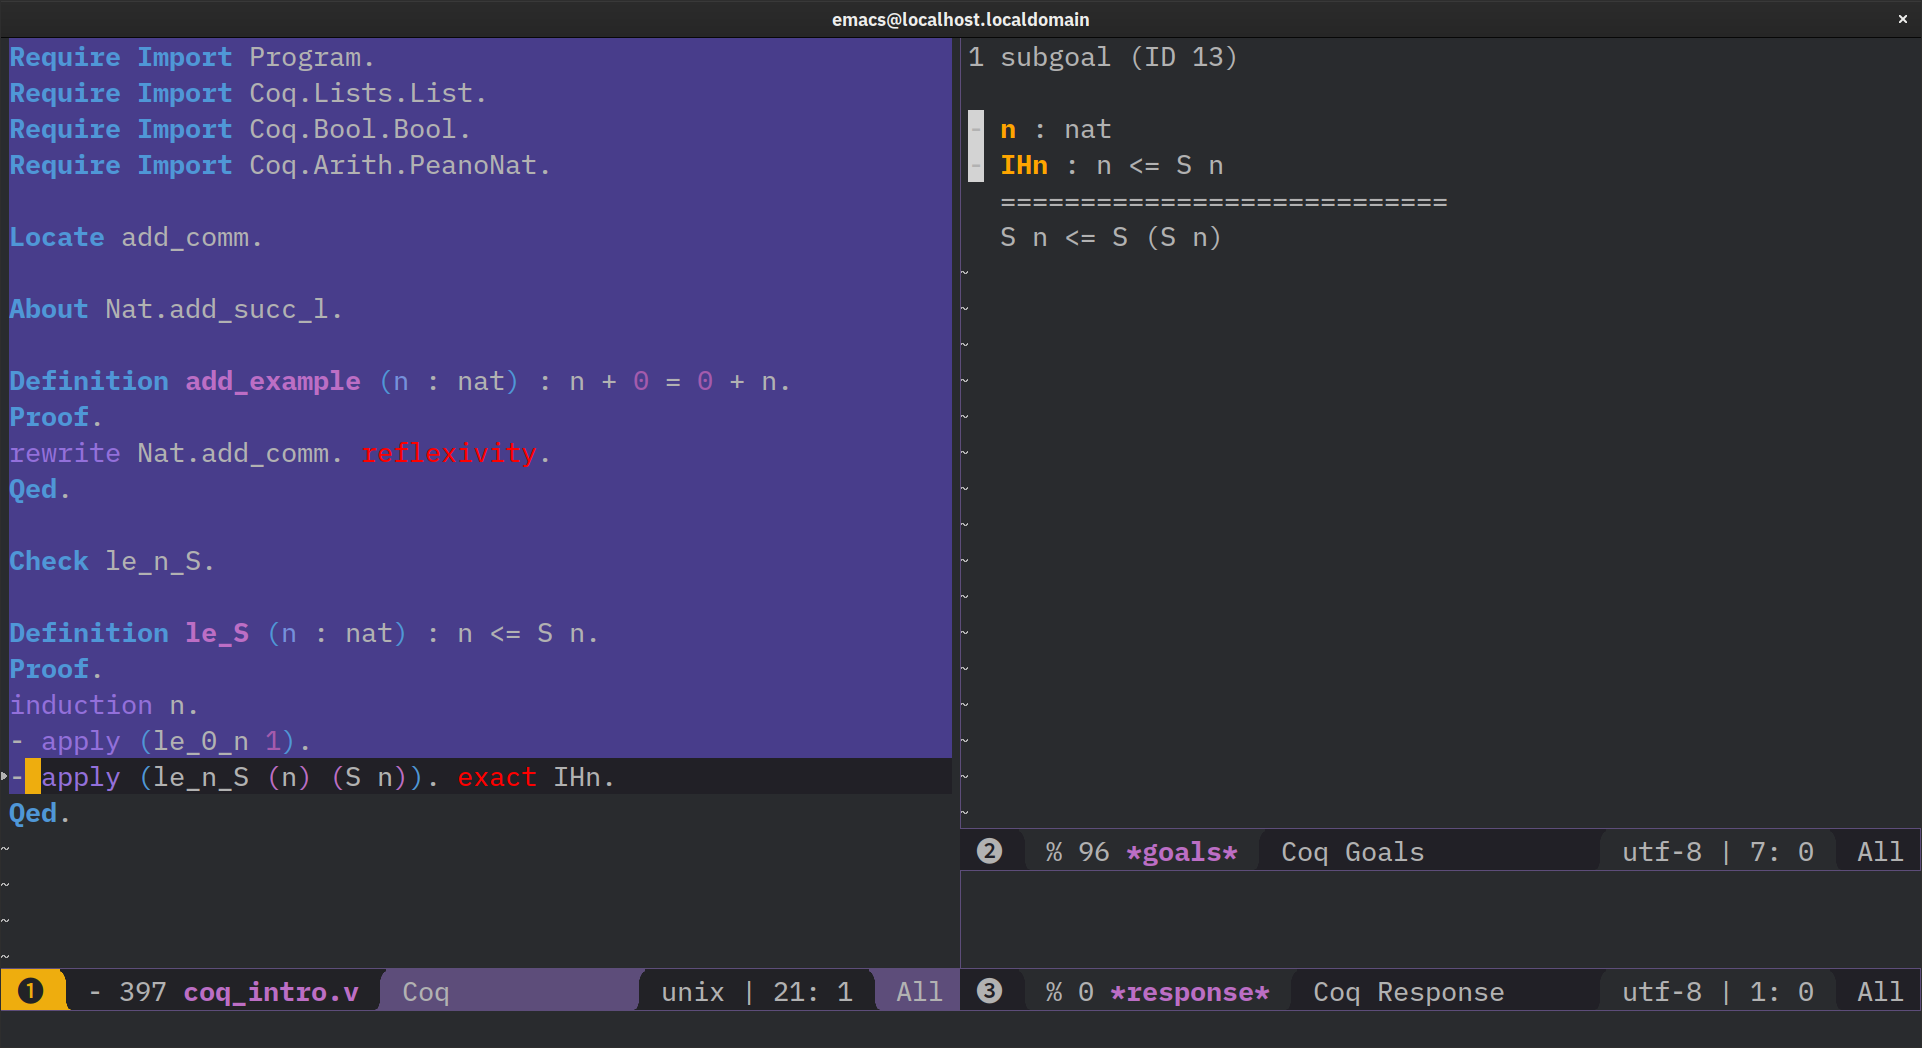
\includegraphics[width=1\textwidth]{gfx/coq_emacs_example.png}
  \caption{Ejemplo de interfaz de Coq}
  \label{fig:ui}
\end{figure}

Coq cuenta con muchos comandos que se usan constantemente. Estos comandos son parte del ``lenguaje'' introducido anteriormente: Vernacular. Algunos de los comandos más importantes son los siguientes.

\begin{description}
  \item[Check] Con \texttt{Check} podemos consultar el tipo de un término. Cuando es llamado en modo prueba, el término es chequeado en el contexto local de la submeta.
  \begin{center}
  \begin{tabular}{| l | l |}
  \hline
  \texttt{Check S O.} & \texttt{S O : nat} \\
  \texttt{Check nat.} & \texttt{Set} \\
  \hline
  \end{tabular}
  \end{center}
  \item[About] El comando \texttt{About} provee información general. Por ejemplo, podemos consultar la signatura de una función, la de un tipo, o consultar el tipo de un constructor. Pero a diferencia de \texttt{Check}, no podemos pasarle cualquier termino. Por ejemplo, \texttt{About S O.} retornará un error.
  \begin{center}
  \begin{tabular}{| l | l |}
  \hline
  \texttt{About S.} & \texttt{S : nat -> nat} \\
  \texttt{About list.} & \texttt{list : Type -> Type} \\
  \hline
  \end{tabular}
  \end{center}
  \item[Print] Podemos pensar a \texttt{Print} como un \texttt{About} que aparte nos muestra la definición completa. Con este podemos inspeccionar elementos ya definidos.
  \begin{center}
  \begin{tabular}{| l | l |}
  \hline
  \texttt{Print list.} & \texttt{Inductive list (A : Type) : Type := ...} \\
  \hline
  \end{tabular}
  \end{center}
  \item[Locate] Con este comando podemos encontrar donde han sido definidos los elementos. 
  \begin{center}
  \begin{tabular}{| l | l |}
  \hline
  \texttt{Locate bool.} & \texttt{Inductive Coq.Init.Datatypes.boo} \\
  \hline
  \end{tabular}
  \end{center}
  \item[Eval] Con \texttt{Eval} podemos evaluar términos. La manera en que los evaluemos o reduzcamos es elegida por nosotros.
  \begin{center}
  \begin{tabular}{| l | l |}
  \hline
  \texttt{Eval compute in 1 + 1.} & \texttt{= 2 : nat} \\
  \texttt{Eval cbv in (fun x => x * (x + 1)) 2.} & \texttt{= 6 : nat} \\
  \hline
  \end{tabular}
  \end{center}
  En este caso \texttt{compute} se traduce a $\beta$-reducir las funciones y \texttt{cbv} se refiere a ``call-by-value''. En este contexto \texttt{compute} y \texttt{cbv} reducen a lo mismo. En otros casos será muy importante diferenciar entre estos, incluyendo \texttt{cbn} (``call-by-name'').
\end{description}

Podemos encontrar una lista completa de estos comandos en \href{https://coq.inria.fr/refman/proof-engine/vernacular-commands.html}{Vernacular Commands}.
